\chapter{Release 2 : Planification Locale et Consolidation Groupe (Sprints 2 et 3)}
\label{chap:sprints_2_3}

\section{Introduction}
Une fois le socle technique et les mécanismes de sécurité validés lors du Sprint 1, l'équipe projet a pu se consacrer au développement du cœur métier de \textit{Cofat Capacity Study}. Cette Release 2, subdivisée en deux Sprints majeurs (Sprint 2 et Sprint 3), constitue la véritable rupture technologique pour les employés du groupe. Dans un premier temps, le Sprint 2 vise à outiller les responsables d'usines (Site Managers) en remplaçant leurs processus manuels par des modules digitaux de planification locale des Équipements, des Espaces et des Ressources Humaines. Nous y détaillerons notamment l'algorithme robuste d'importation de fichiers Excel. Dans un second temps, le Sprint 3 exploite l'architecture centralisée de la base de données pour générer, à la volée, les consolidations à l'échelle mondiale de ces mêmes entités (Cofat Group). Ce chapitre abordera enfin la mise en place du référentiel \textit{StandardInvestment V2}, outil décisif pour l'évaluation des futurs investissements industriels du Groupe COFAT.

Sur le plan méthodologique, cette Release 2 a représenté la charge de développement la plus importante du projet en nombre de lignes de code produites, les trois modules de planification locale (Équipements, Espaces, RH) partageant une architecture technique commune mais nécessitant chacun une logique métier, une structure de tableau et un jeu de règles de validation spécifiques. Le choix a été fait de développer ces trois modules de façon strictement séquentielle plutôt qu'en parallèle, chaque module bénéficiant des retours d'expérience techniques accumulés sur le précédent : la logique de code couleur et de filtrage dynamique développée pour le module Équipements a par exemple directement inspiré l'ergonomie retenue pour les deux modules suivants, garantissant une cohérence visuelle et fonctionnelle perçue par l'utilisateur final comme un ensemble unifié plutôt que comme trois outils juxtaposés.

\section{Sprint 2 : Déploiement des modules de Planification Locale}
La planification locale est l'action par laquelle chaque usine projette ses besoins capacitaires en fonction des commandes automobiles à venir. L'objectif de ce sprint était de numériser cette étape de manière transparente, en conservant la souplesse d'Excel tout en apportant la rigueur d'une base de données relationnelle.

\subsection{Backlog et critères d'acceptation du Sprint 2}
Le Sprint 2, déroulé de mai à juin 2026, a pris en charge les User Stories US-04 à US-07 du Backlog Général présenté au chapitre 2, toutes rattachées au profil Site Manager. Le tableau \ref{tab:backlog_sprint2} rappelle leur description et précise, pour chacune, les critères d'acceptation qui ont guidé les tests de recette effectués lors de la Sprint Review.

\begin{table}[h]
\centering
\begin{tabular}{|p{1.6cm}|p{6cm}|p{7cm}|}
\hline
\textbf{ID US} & \textbf{Description} & \textbf{Critère d'acceptation principal} \\ \hline
US-04 & Importer un fichier Excel des équipements locaux & Les lignes invalides (types incorrects, colonnes manquantes) doivent être rejetées individuellement sans bloquer l'import des lignes valides du même fichier \\ \hline
US-05 & Visualiser l'analyse de charge (Load \%) & Le code couleur (vert/orange/rouge) doit se recalculer automatiquement dès qu'une valeur de \texttt{machineNeed} ou \texttt{availableMachine} est modifiée, sans rechargement de page \\ \hline
US-06 & Importer et analyser les besoins RH & La matrice temporelle (12 mois + 8 trimestres) doit rester lisible et navigable au clavier comme à la souris sur un écran de résolution standard bureau \\ \hline
US-07 & Importer et gérer les espaces de production & Le graphique de taux d'occupation doit se mettre à jour immédiatement après la validation d'un nouvel import, sans nécessiter d'action supplémentaire de l'utilisateur \\ \hline
\end{tabular}
\caption{Backlog et critères d'acceptation du Sprint 2}
\label{tab:backlog_sprint2}
\end{table}

\subsection{Le Module des Équipements Industriels}
L'objectif du module "Équipements" est de permettre au Site Manager de suivre l'état de saturation de son parc de machines (presses, coupeuses, soudeuses) et d'identifier rapidement les goulots d'étranglement qui pourraient bloquer la production d'un nouveau projet automobile.

Avant l'interface, le Site Manager calcule théoriquement le besoin. Il le saisit ensuite dans l'application ou l'importe (nous verrons l'import plus bas).

\vspace{0.5cm}
\begin{figure}[H]
    \centering
    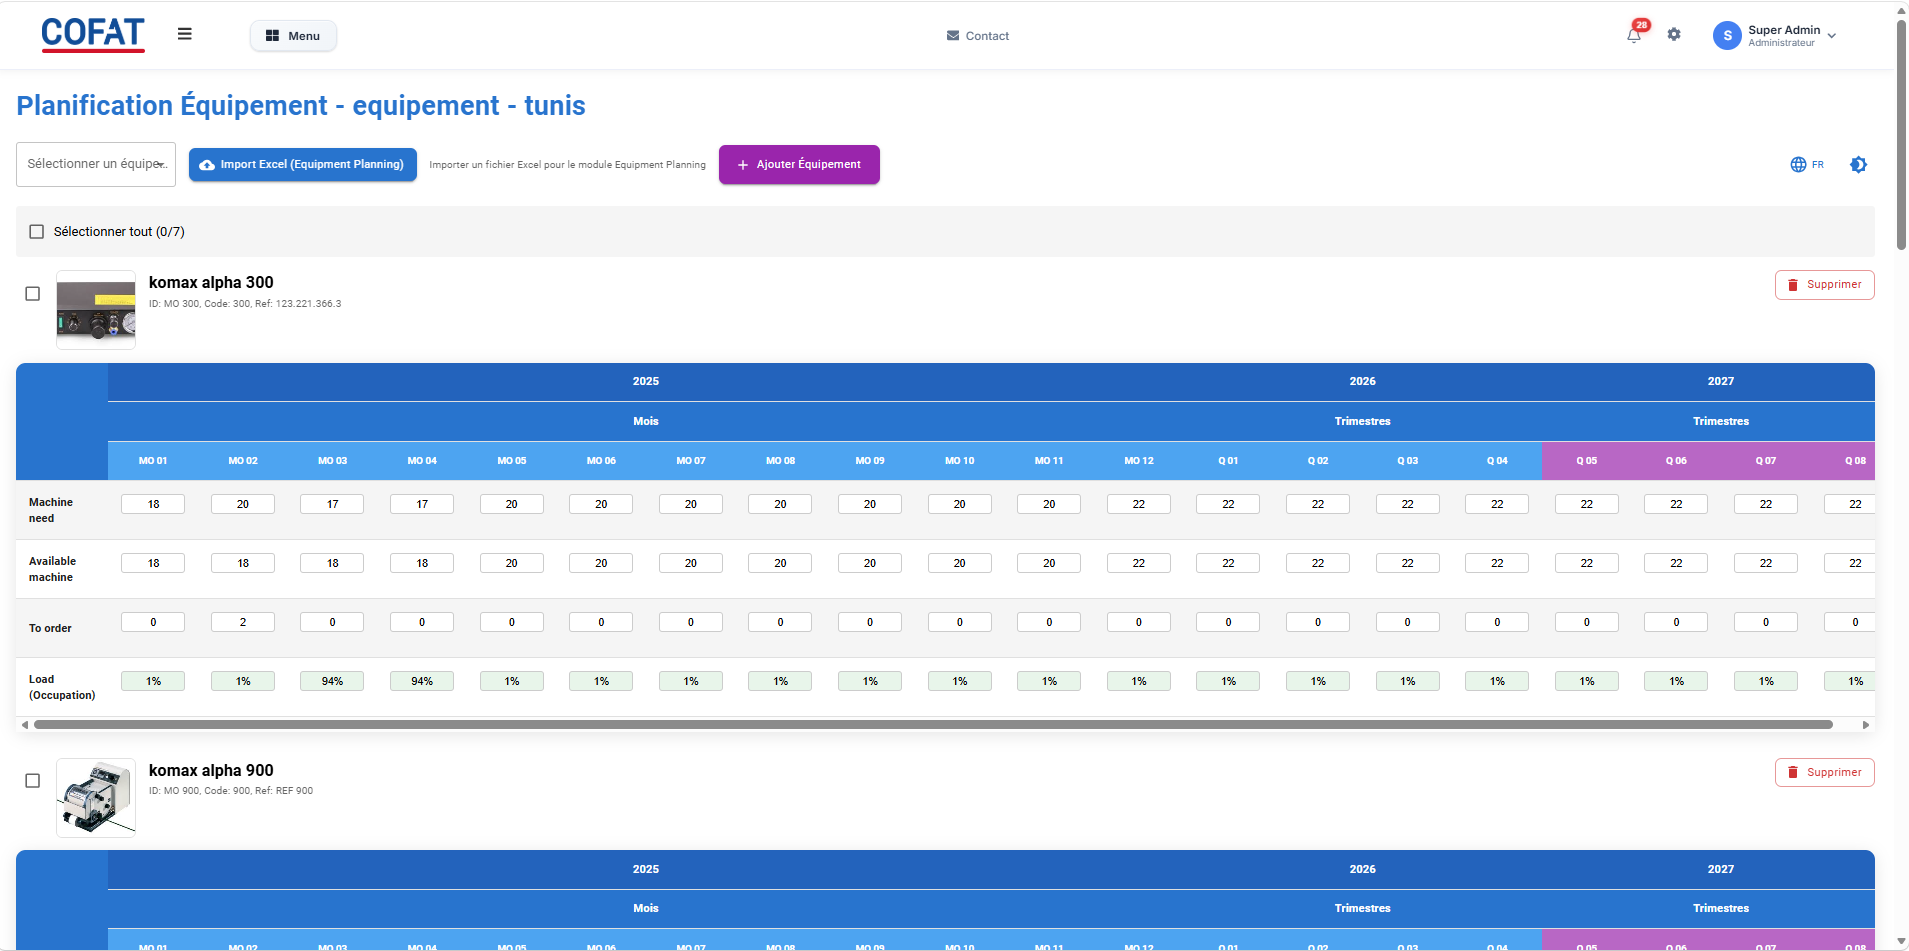
\includegraphics[width=1\textwidth]{img/planification equipement standard.png}
    \caption{Interface de planification locale des équipements}
    \label{fig:planif_equipement}
\end{figure}
\vspace{0.5cm}

\textbf{Analyse détaillée de l'interface (Figure \ref{fig:planif_equipement}) :}
La conception de cette interface a privilégié la clarté visuelle, car l'ingénieur méthodes doit scanner des dizaines de lignes en un clin d'œil. Le tableau de données, implémenté avec Material UI (DataGrid), présente les colonnes suivantes :
\begin{itemize}
    \item \textbf{Type d'Équipement} : La désignation de la machine (ex: Komax Alpha 530).
    \item \textbf{Opération} : L'application permet un filtrage dynamique par étape de production. L'utilisateur peut isoler les machines de la zone "1-COUPE", "2-PREPARATION", "3-ASSEMBLAGE" ou "4-CONTROLE ELECTRIQUE ET CONDITIONNEMENT".
    \item \textbf{machineNeed} : Le besoin calculé par l'ingénieur (par exemple 4.5 machines requises pour absorber le volume).
    \item \textbf{availableMachine} : Le parc physique réel sur le site (par exemple 4 machines).
    \item \textbf{load (\%)} : C'est le taux de charge, métrique fondamentale. Il est calculé algorithmiquement par le frontend React (et vérifié par le backend) selon la formule $Load = (machineNeed / availableMachine) \times 100$. Un code couleur visuel (conditional formatting) alerte immédiatement l'ingénieur :
        \begin{itemize}
            \item \textbf{Vert (Load $\le$ 80\%)} : Sous-charge, l'usine a de la marge.
            \item \textbf{Orange (80\% $<$ Load $\le$ 100\%)} : Zone de tension, l'équipement est optimisé au maximum.
            \item \textbf{Rouge (Load $>$ 100\%)} : Surcharge critique. Dans notre exemple (4.5 / 4), le load de 112.5\% s'affiche en rouge vif.
        \end{itemize}
    \item \textbf{toOrder} : Ce champ calcule le déficit. Si le load dépasse 100\%, il indique le nombre d'unités manquantes (ici 0.5, arrondi au supérieur pour la commande).
\end{itemize}

\textbf{Justification du code couleur à trois niveaux :} le choix de fixer le seuil d'alerte "orange" à 80\% plutôt qu'à 100\% n'est pas arbitraire. Il reflète une pratique industrielle standard consistant à anticiper la saturation avant qu'elle ne devienne critique : une machine fonctionnant en permanence à un taux de charge proche de 100\% ne dispose plus d'aucune marge pour absorber les aléas de production (pannes, maintenance préventive, absentéisme), alors qu'un signal visuel dès 80\% laisse le temps au Site Manager d'anticiper une commande ou un transfert de machine avant que la situation ne devienne bloquante pour la ligne de production. Ce seuil de 80\%, ainsi que la formule de calcul du \textit{Load}, avaient déjà cours dans les anciens fichiers Excel décrits au chapitre 1 ; l'application ne fait ici que fiabiliser et automatiser un calcul métier préexistant, ce qui a grandement facilité l'adoption de l'outil par les ingénieurs méthodes, déjà familiers avec cette logique.

Le filtre dynamique par opération (1-COUPE, 2-PREPARATION, 3-ASSEMBLAGE, 4-CONTROLE ELECTRIQUE ET CONDITIONNEMENT) est implémenté côté frontend sous forme de composant \textit{Tabs} de Material UI, chaque onglet déclenchant un nouvel appel à l'API filtré par le paramètre de requête correspondant (\texttt{GET /api/equipment/planning?operation=COUPE}), plutôt qu'un filtrage côté client sur l'intégralité des données déjà chargées. Ce choix, bien que plus coûteux en nombre de requêtes réseau, garantit que le Site Manager d'un site comportant plusieurs centaines de lignes d'équipements ne voit jamais son navigateur ralentir au chargement initial de la page.

\subsection{Le Module d'analyse de l'Occupation des Espaces}
L'espace physique (surface au sol en m²) est une contrainte dure dans une usine de câblage. Une ligne d'assemblage ne peut pas être superposée. Le module "Espaces" permet d'avoir une vision cartographiée et quantitative de la surface disponible pour accueillir de futurs projets.

\vspace{0.5cm}
\begin{figure}[H]
    \centering
    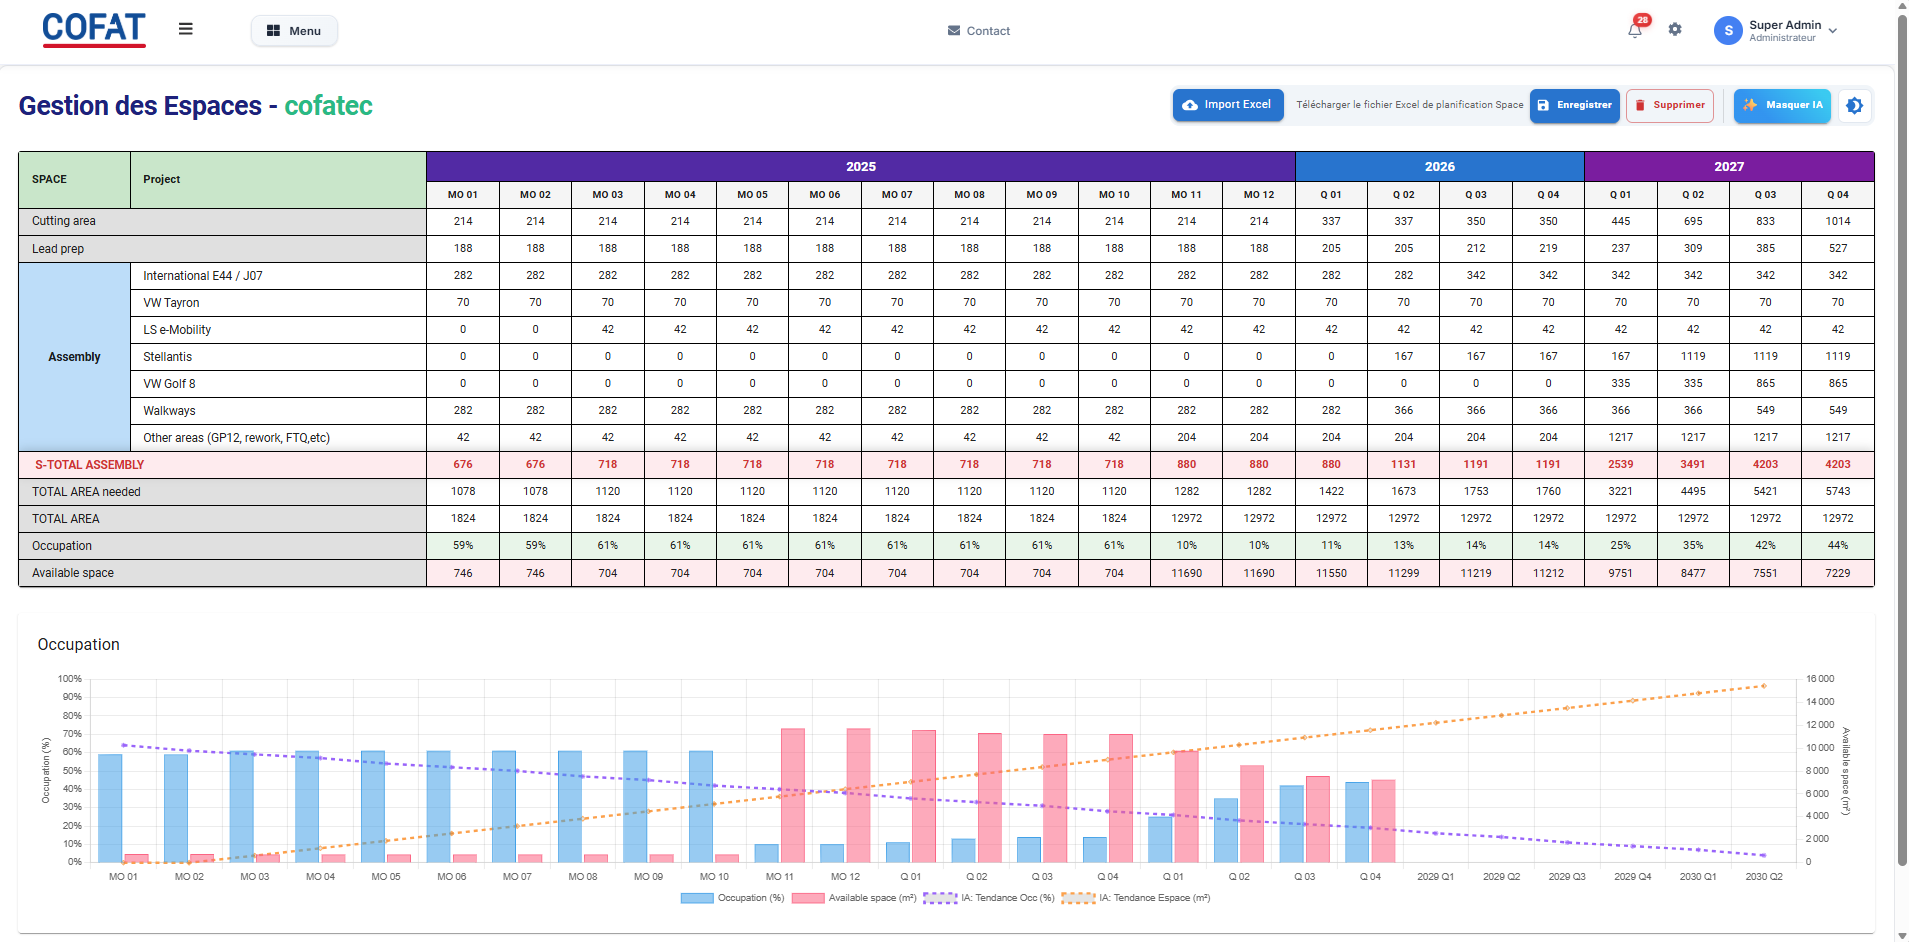
\includegraphics[width=0.9\textwidth]{img/analyse des espaces.png}
    \caption{Tableau de gestion des surfaces par zone de production}
    \label{fig:tableau_espaces}
\end{figure}
\vspace{0.5cm}

\vspace{0.5cm}
\begin{figure}[H]
    \centering
    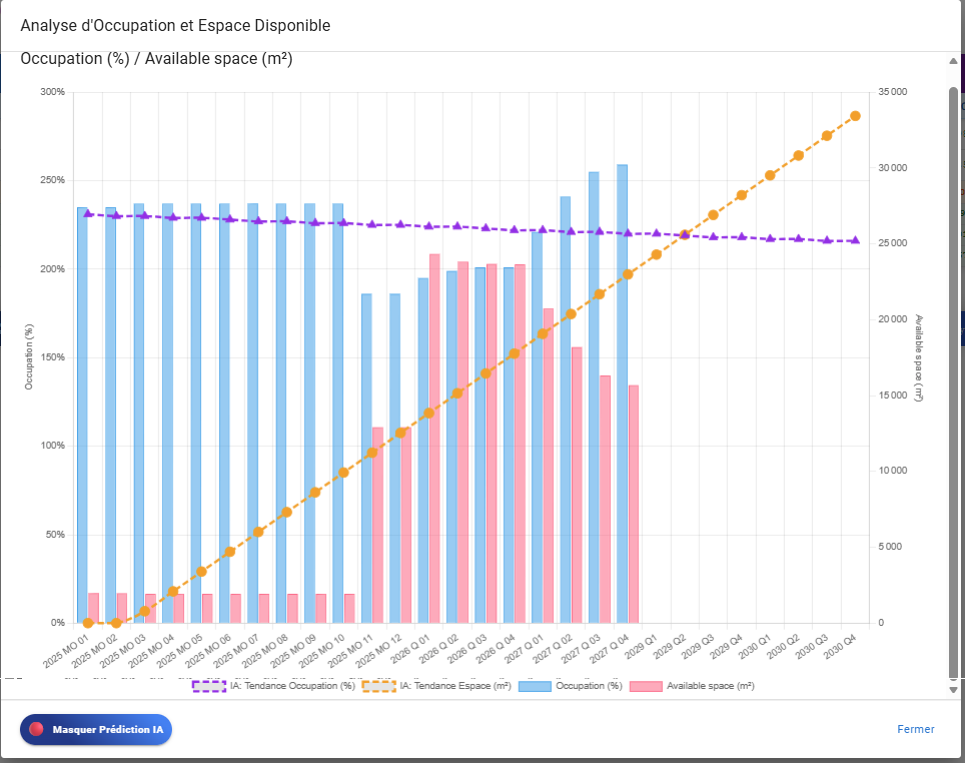
\includegraphics[width=0.9\textwidth]{img/analyse d'occupation et espace disponible.png}
    \caption{Tableau de bord visuel : Taux d'occupation global du site}
    \label{fig:graphique_espaces}
\end{figure}
\vspace{0.5cm}

\textbf{Analyse du fonctionnement du module Espaces :}
Comme illustré dans la Figure \ref{fig:tableau_espaces}, l'interface sépare l'usine en grandes zones logiques. On y retrouve les zones de traitement primaire (\textit{coupe}, \textit{préparation}) et les vastes halls dédiés aux projets clients majeurs (visibles dans l'interface : \textit{VW Tayron}, \textit{International E44}, \textit{Stellantis J4U}, \textit{VW Golf 8}, \textit{LS e-mobility BEV-A}). 

Pour chaque zone, l'ingénieur déclare la surface totale et la surface occupée. La Figure \ref{fig:graphique_espaces} met en évidence la puissance de la bibliothèque \textit{Charts.js}. Le composant React extrait ces données et génère un diagramme circulaire (Pie Chart) montrant, d'un coup d'œil, le ratio Espace Occupé / Espace Libre pour l'usine entière. Ce graphique interactif aide le directeur de site à décider rapidement s'il peut accepter la ligne de production d'un nouveau modèle de véhicule ou s'il doit louer une extension de bâtiment.

\textbf{Pourquoi une gestion par zone plutôt qu'une surface globale unique ?} Le découpage par zone logique (coupe, préparation, puis un hall dédié par projet client) reflète directement l'organisation physique réelle d'une usine COFAT, où chaque ligne de production est physiquement cloisonnée pour des raisons de sécurité et de flux logistique (éviter le croisement des flux de pièces entre projets). Un simple indicateur de surface globale disponible aurait masqué une information pourtant critique pour la décision : une usine peut afficher un taux d'occupation global de 60\% tout en étant dans l'incapacité totale d'accueillir un nouveau projet, si les 40\% de surface restante sont fragmentés entre plusieurs petites zones non contiguës et physiquement incompatibles avec l'implantation d'une nouvelle ligne d'assemblage. La granularité par zone du module permet à l'ingénieur méthodes de répondre précisément à cette question avant de s'engager auprès d'un client.

\subsection{Le Module de prévision des Ressources Humaines (RH)}
Le recrutement et la formation des opérateurs prennent des semaines. Le module RH permet d'anticiper les embauches sur un horizon de trois ans, répartis par catégories et par projets de véhicules.

\vspace{0.5cm}
\begin{figure}[H]
    \centering
    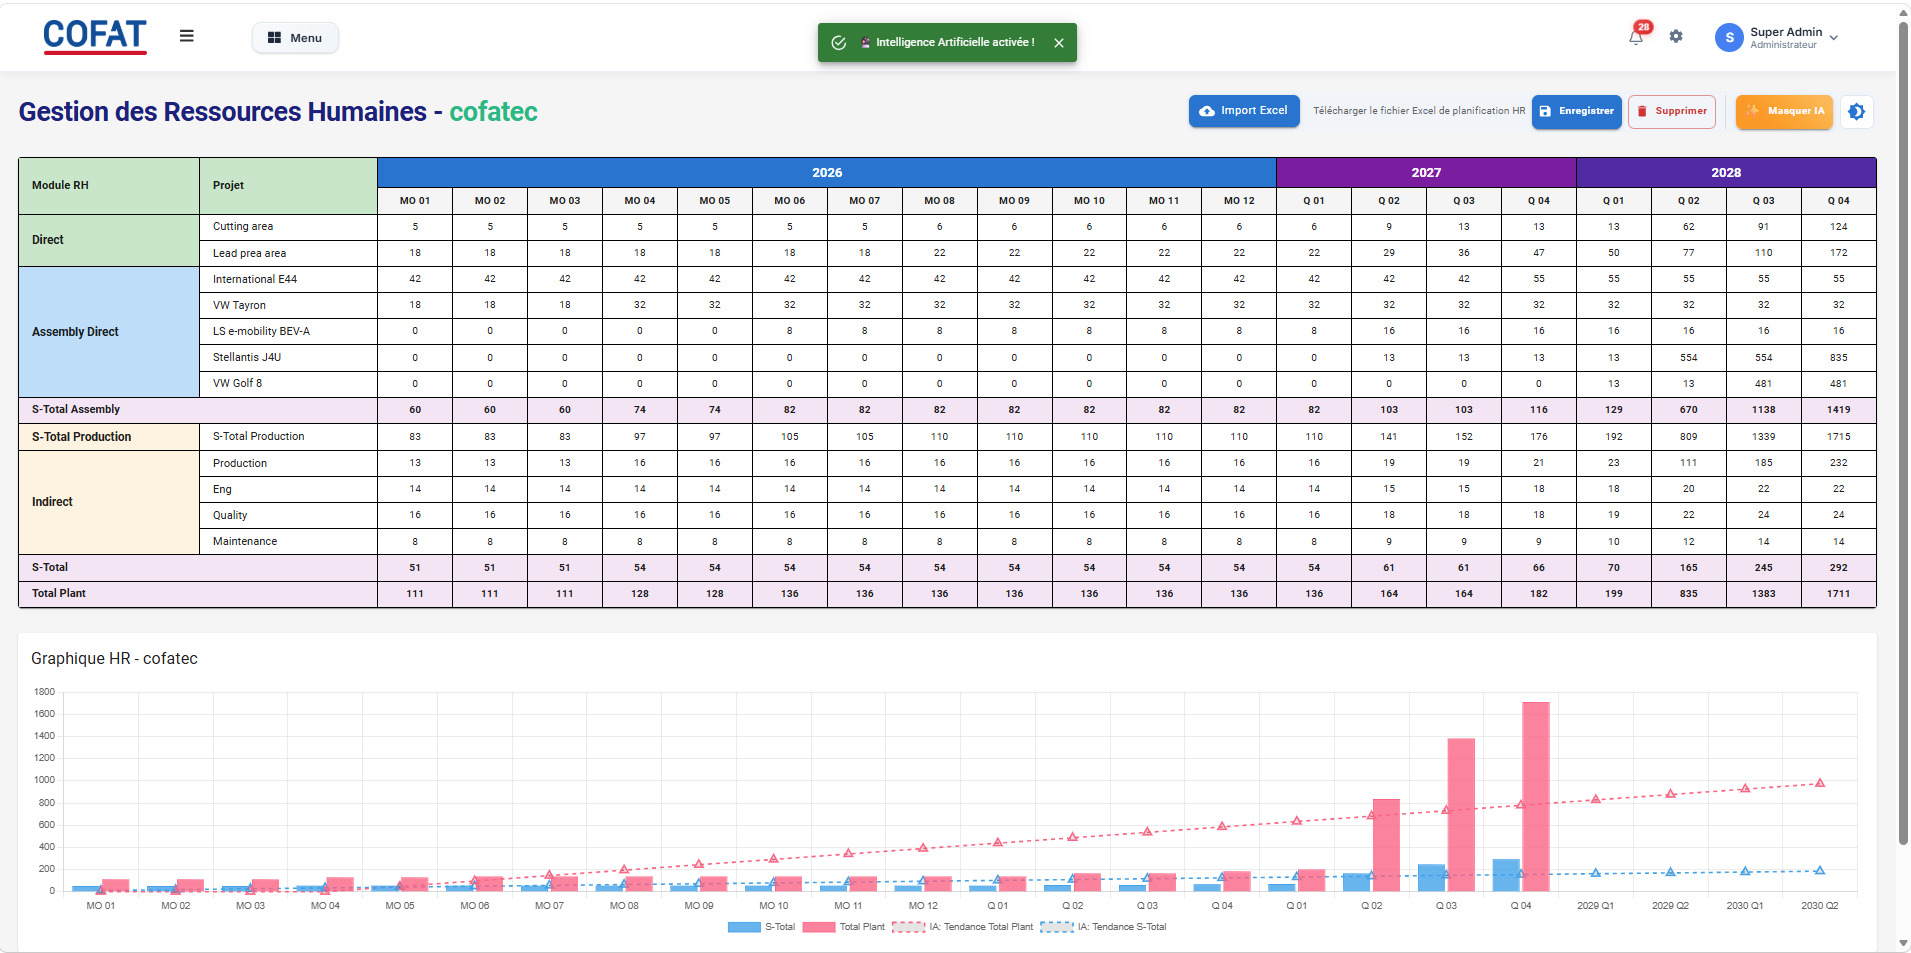
\includegraphics[width=1\textwidth]{img/gestion des resources humaines.png}
    \caption{Interface de planification temporelle des Ressources Humaines}
    \label{fig:planif_rh}
\end{figure}
\vspace{0.5cm}

\textbf{Analyse de la matrice temporelle RH (Figure \ref{fig:planif_rh}) :}
Ce module a été le plus complexe à modéliser ergonomiquement, car il présente une dimension temporelle très étendue. Le tableau de données, généré dynamiquement par un composant Ant Design, croise la dimension "Métier" avec la ligne de temps :
\begin{itemize}
    \item \textbf{Structuration en lignes} : Les effectifs sont regroupés par grandes catégories : \textit{Direct} (opérateurs machines), \textit{Indirect} (qualité, maintenance, logistique), et \textit{Assemblage Direct}. L'interface décline ensuite ces catégories par sous-projets (\textit{Cutting area}, \textit{Lead prea area}, et les projets d'assemblage comme \textit{VW Tayron} ou \textit{Stellantis J4U}).
    \item \textbf{Structuration en colonnes (Time-Series)} : Pour offrir une vision de \textit{ramp-up} (montée en cadence), le système affiche la prévision mensuelle pour l'année courante (colonnes MO 01 à MO 12 pour 2025), puis bascule sur une granularité trimestrielle pour les années futures (colonnes Q01 à Q04 pour 2026 et 2027).
\end{itemize}
Le système compare en permanence ces prévisions au \textit{Headcount} (effectif actuel) et calcule les écarts d'embauche.

\textbf{Justification du choix d'une granularité temporelle variable :} le passage d'une vision mensuelle pour l'année courante (2025) à une vision trimestrielle pour les années suivantes (2026-2027) n'est pas un artifice technique mais reflète une réalité de gestion des ressources humaines partagée par l'ensemble des Site Managers consultés lors de la phase de spécification. À court terme, la précision mensuelle est indispensable pour piloter finement les campagnes de recrutement en cours, dont les délais (publication d'offre, entretiens, période de préavis du candidat, formation initiale) se comptent en semaines. À plus long terme en revanche, une précision mensuelle sur trois années à venir aurait donné une illusion de certitude sur des données par nature volatiles, les volumes de commande des constructeurs automobiles n'étant contractuellement confirmés qu'à l'horizon d'un ou deux trimestres. La granularité trimestrielle pour 2026-2027 reflète donc fidèlement le niveau de certitude réel de la donnée business sous-jacente, évitant de suggérer une fausse précision aux décideurs RH du groupe.

Sur le plan technique, cette double granularité a nécessité une modélisation particulière de la table \texttt{HR} : plutôt que de créer une colonne SQL dédiée pour chacune des 20 périodes (ce qui aurait rigidifié le schéma en cas d'évolution future du découpage temporel), chaque ligne de la table représente une période unique identifiée par un champ \texttt{period} (par exemple "MO\_01\_2025" ou "Q02\_2026"), le frontend React se chargeant de pivoter dynamiquement ces lignes en colonnes lors de l'affichage matriciel. Cette approche, bien que légèrement plus coûteuse en nombre de lignes stockées, offre une flexibilité précieuse : faire évoluer demain la granularité (par exemple, passer à une vision mensuelle sur 2026 également) ne nécessiterait aucune migration de schéma, uniquement une adaptation du code de génération des périodes.

\subsection{L'Ingénierie de l'Import Excel (Le cœur de la saisie de données)}
Saisir à la main des dizaines de cellules RH (12 mois + 8 trimestres par projet) dans un formulaire web aurait provoqué un rejet immédiat de l'application par les ingénieurs. C'est pourquoi j'ai développé un algorithme d'importation massive depuis des fichiers Excel (.xlsx).

\textbf{Le processus technique détaillé (\textit{Data Pipeline}) :}
\begin{enumerate}
    \item \textbf{Côté React (Frontend)} : L'utilisateur clique sur le bouton "Importer Excel". Un élément \texttt{<input type="file">} s'ouvre. Une fois le fichier sélectionné, le navigateur lit le fichier avec l'API HTML5 \texttt{FileReader}. Le contenu est inséré dans un objet \texttt{FormData} et envoyé au serveur via une requête \texttt{POST} Axios en \texttt{multipart/form-data}.
    \item \textbf{Côté Express (Middleware Multer)} : À l'arrivée sur le port 9001, le middleware \texttt{multer} intercepte le flux binaire. Il sauvegarde temporairement le fichier dans le dossier \texttt{/uploads/budget} (ou \texttt{/uploads/hr}).
    \item \textbf{Côté Node.js (Parsing avec XLSX)} : Le script de contrôleur prend le relais. Il utilise la bibliothèque \texttt{xlsx} (SheetJS) pour parser le buffer (\textit{ArrayBuffer}). Le code convertit la première feuille (Worksheet) du classeur en un tableau d'objets JSON (\texttt{XLSX.utils.sheet\_to\_json()}).
    \item \textbf{Logique de Validation} : C'est ici que l'application prouve sa supériorité. Le script Node parcourt le tableau JSON et valide \textbf{chaque colonne}. Par exemple, si une cellule \texttt{machineNeed} contient du texte au lieu d'un nombre, ou si une ligne est entièrement vide, l'algorithme nettoie ou rejette la ligne de manière chirurgicale, en renvoyant un tableau des erreurs au frontend (ex: "Erreur Ligne 45: Valeur 'abc' invalide pour MO 03").
    \item \textbf{Insertion Massive (Sequelize bulkCreate)} : Si les données sont intègres, Sequelize exécute une fonction \texttt{bulkCreate()}, insérant les centaines de lignes dans la base SQL Server en une seule transaction ACID optimisée, garantissant qu'il n'y ait pas de doublons. En cas de succès, le fichier temporaire est supprimé du serveur et le frontend affiche un toast de réussite (SweetAlert2).
\end{enumerate}

\vspace{0.5cm}
\begin{figure}[H]
    \centering
    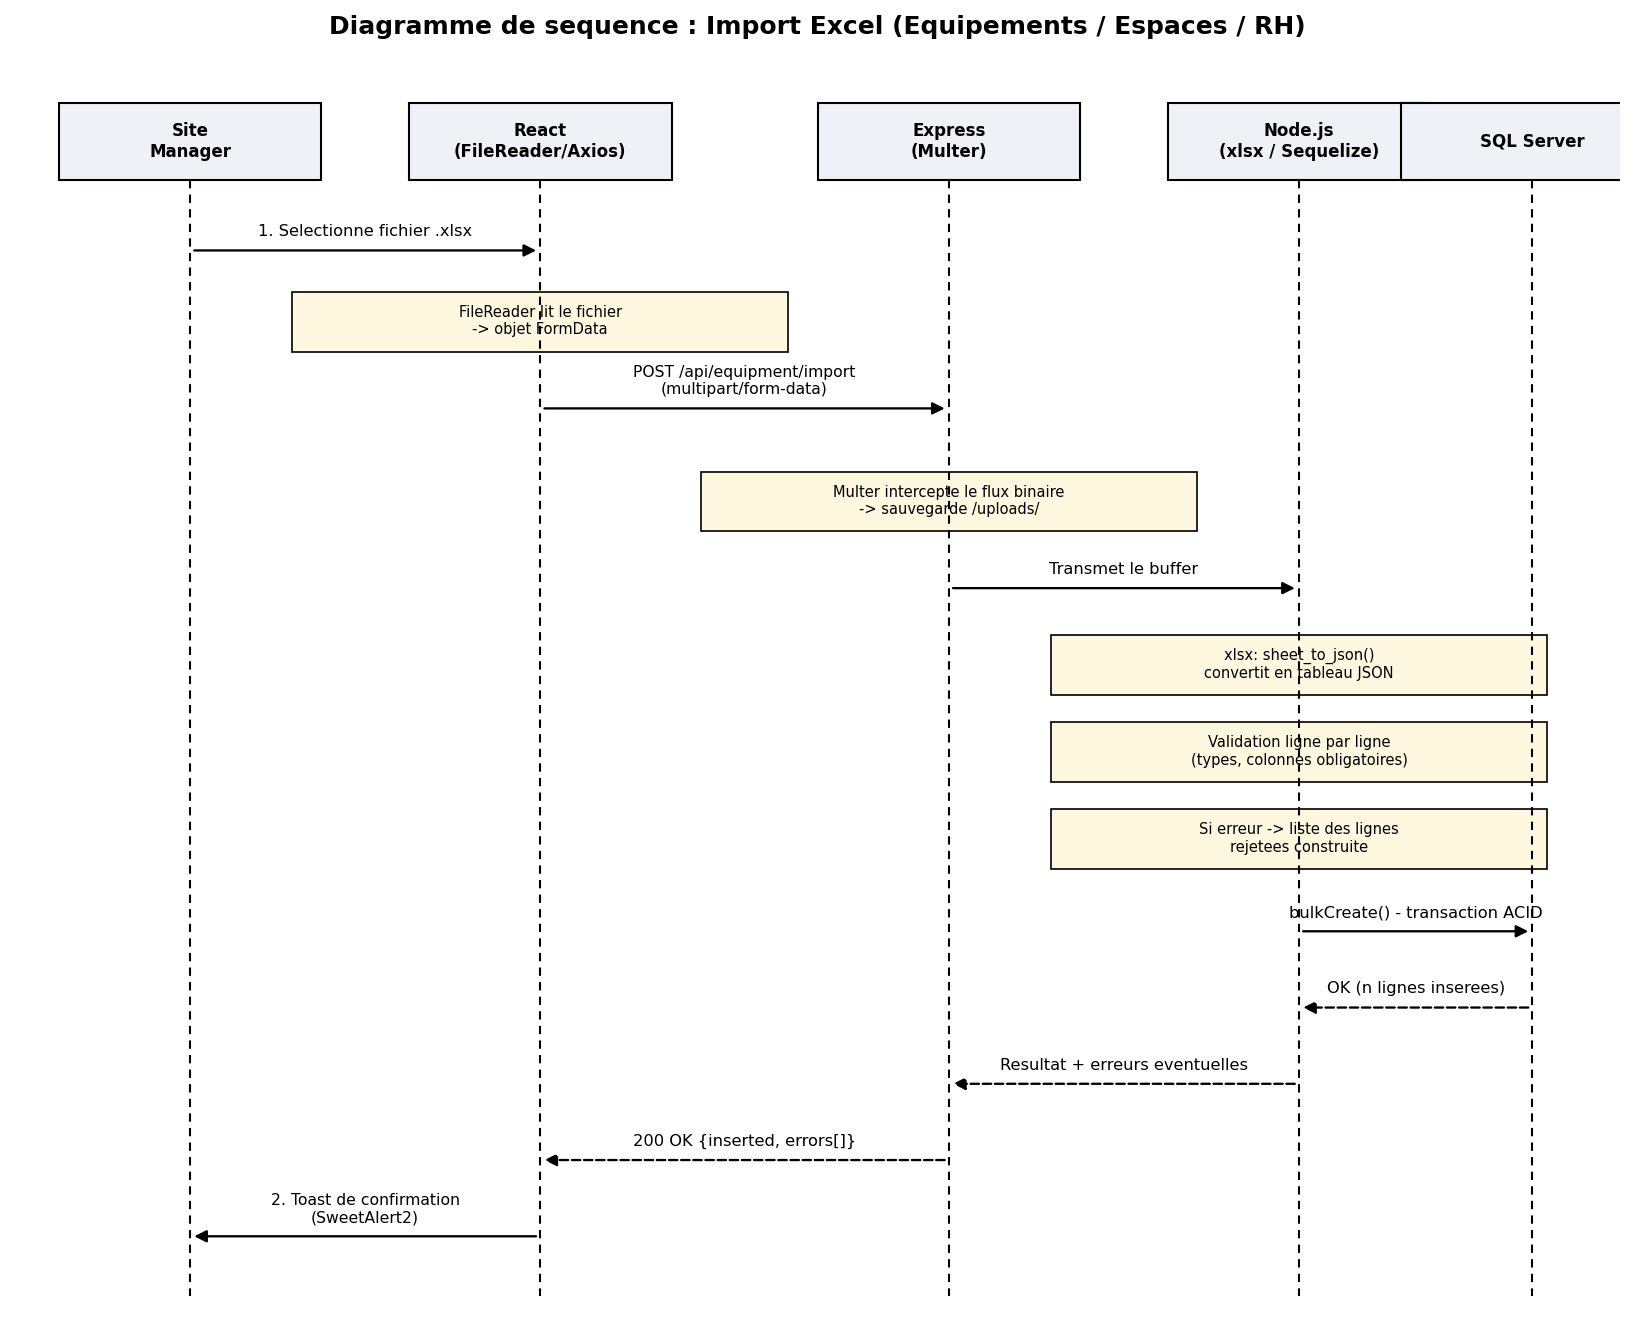
\includegraphics[width=1\textwidth]{img/seq_import_excel.png}
    \caption{Diagramme de séquence du processus d'import Excel}
    \label{fig:seq_import}
\end{figure}
\vspace{0.5cm}

\textbf{Lecture du diagramme (Figure \ref{fig:seq_import}) :} ce diagramme met en évidence un point d'architecture important : le fichier Excel transite physiquement par le serveur (répertoire \texttt{/uploads/}) avant d'être parsé, plutôt que d'être traité entièrement en mémoire. Ce choix, bien que consommant temporairement de l'espace disque, protège le serveur Node.js contre une saturation de la mémoire vive (RAM) dans le cas où un utilisateur importerait, par erreur, un fichier Excel volumineux de plusieurs dizaines de milliers de lignes. Le fichier temporaire est systématiquement supprimé du serveur une fois le traitement terminé, qu'il ait réussi ou échoué, afin de ne jamais laisser d'artefact résiduel sur le disque du serveur de production.

\textbf{Robustesse face aux fichiers hétérogènes :} dans la pratique, les fichiers Excel envoyés par les dix sites du groupe ne sont jamais parfaitement homogènes — certains ingénieurs ajoutent des colonnes de commentaires personnels, d'autres laissent des lignes de total en bas de leur tableau, hérité de leurs anciennes habitudes de travail. L'algorithme de validation a donc été conçu pour être tolérant sur la forme (il ignore les colonnes inconnues et les lignes ne correspondant à aucun schéma de données attendu) mais strict sur le fond (toute valeur numérique attendue mais absente ou non conforme est explicitement signalée dans le rapport d'erreurs retourné à l'utilisateur), un compromis qui s'est révélé indispensable après les premiers tests réalisés avec de véritables fichiers issus du site de Mateur lors de la Sprint Review du Sprint 2.

\section{Sprint 3 : La Consolidation Mondiale (Cofat Group)}
Si la planification locale (Sprint 2) permet aux usines de respirer, c'est le module de Consolidation Groupe (Sprint 3) qui donne à la Direction (Admin) le véritable retour sur investissement du projet. 
Avant ce sprint, réunir les 10 entités de 6 pays différents prenait des jours de manipulation Excel. Désormais, le simple accès à l'onglet "Cofat Group" exécute des requêtes SQL d'agrégation massives qui produisent un état des lieux mondial en moins de trois secondes.

\subsection{Backlog et critères d'acceptation du Sprint 3}
Le Sprint 3, déroulé en juillet 2026, a pris en charge les User Stories US-08 à US-10, exclusivement rattachées au profil Administrateur (à l'exception de la mise à jour des coûts par l'Achat sur le catalogue). Le tableau \ref{tab:backlog_sprint3} en détaille les critères d'acceptation.

\begin{table}[h]
\centering
\begin{tabular}{|p{1.6cm}|p{6cm}|p{7cm}|}
\hline
\textbf{ID US} & \textbf{Description} & \textbf{Critère d'acceptation principal} \\ \hline
US-08 & Visualiser le dashboard consolidé mondial des Équipements & Le total consolidé affiché doit être strictement égal à la somme exacte des valeurs des 10 sites au moment de la requête, vérifiable manuellement lors de la recette \\ \hline
US-09 & Visualiser la consolidation des Espaces et RH du groupe & Les graphiques doivent rester exploitables (lisibles, non tronqués) même avec l'intégralité des 10 sites affichés simultanément \\ \hline
US-10 & Consulter et mettre à jour les coûts du catalogue StandardInvestment & Seul le champ de coût doit être éditable par le rôle Achat ; toute tentative de modification d'un autre champ par ce rôle doit être silencieusement ignorée côté serveur \\ \hline
\end{tabular}
\caption{Backlog et critères d'acceptation du Sprint 3}
\label{tab:backlog_sprint3}
\end{table}

\subsection{Consolidation des Équipements}
La logique d'agrégation métier est puissante. La base SQL Server contient les besoins de l'usine de Mateur (Tunisie), de São Paulo (Brésil) et de Durango (Mexique).

\vspace{0.5cm}
\begin{figure}[H]
    \centering
    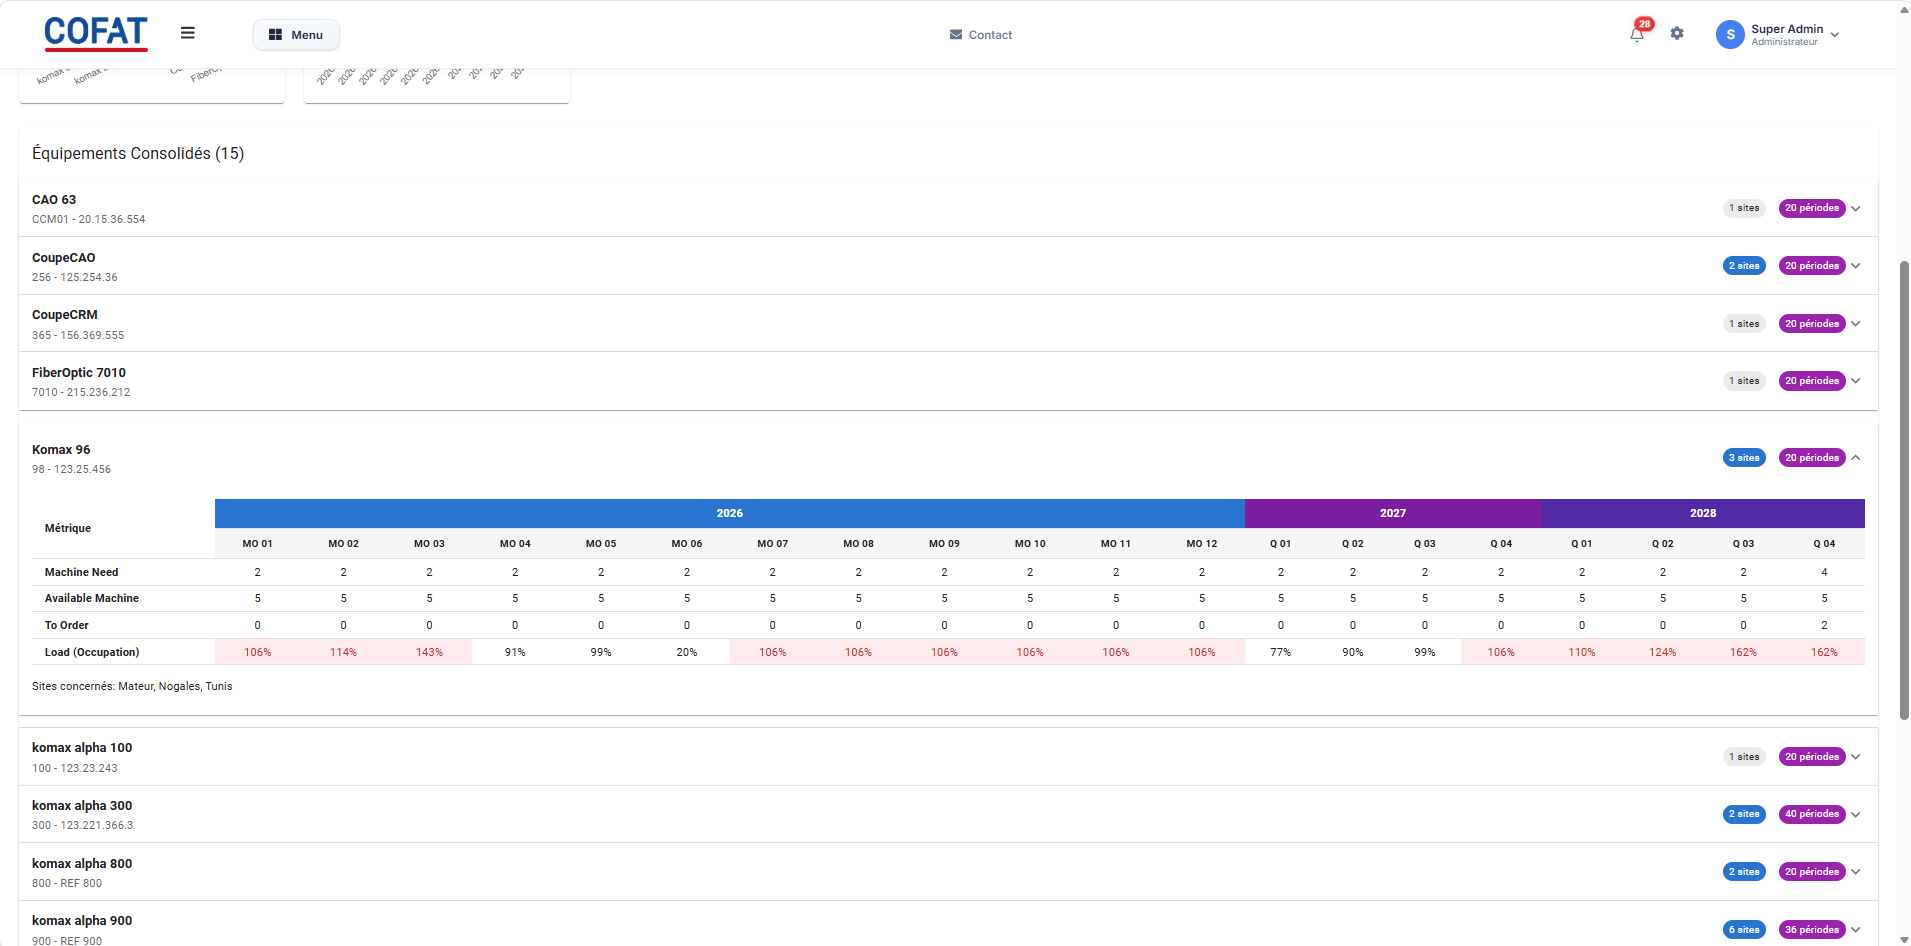
\includegraphics[width=0.9\textwidth]{img/consolidatinon cofatgroup Equipment.png}
    \caption{Tableau de consolidation mondiale des équipements industriels}
    \label{fig:conso_equipements}
\end{figure}
\vspace{0.5cm}

\textbf{L'algorithme d'agrégation (Figure \ref{fig:conso_equipements}) :}
L'API Node.js exécute une requête Sequelize utilisant les fonctions d'agrégation natives du SGBD (\texttt{sequelize.fn('SUM')}). La requête groupe les données par \textit{Type d'équipement} (\texttt{GROUP BY equipmentId}) et somme les champs \texttt{machineNeed} et \texttt{availableMachine} de \textbf{tous} les sites. 
Le résultat est éclatant pour le Backoffice : si l'usine du Mexique déclare un besoin urgent (toOrder = +2) sur une machine Komax, et que l'usine d'Égypte déclare un surplus sur ce même modèle (toOrder = -2), le tableau consolidé affichera un \textit{toOrder mondial} de zéro. La direction saura immédiatement qu'au lieu d'acheter deux machines neuves, elle doit simplement ordonner le transfert physique des machines d'Égypte vers le Mexique, économisant ainsi des centaines de milliers d'euros en une seule vue logicielle.

\textbf{Considérations de performance :} l'exigence non fonctionnelle du chapitre 2 imposait un temps de réponse inférieur à 3 secondes pour cette agrégation portant sur dix sites. Pour y parvenir, les colonnes \texttt{siteId} et \texttt{equipmentId} de la table \texttt{EquipmentPlanning} sont indexées au niveau SQL Server, ce qui permet au moteur de requête d'éviter un parcours complet de la table (\textit{full table scan}) lors du \texttt{GROUP BY}. De plus, la requête d'agrégation est exécutée directement au niveau du SGBD via les fonctions natives de Sequelize plutôt que d'être recalculée en JavaScript après récupération de la totalité des lignes brutes, ce qui délègue le calcul lourd au moteur SQL Server, historiquement optimisé pour ce type d'opération ensembliste.

\subsection{Consolidation des Espaces et des RH}
Le même principe d'agrégation mathématique est appliqué aux surfaces industrielles et aux effectifs.

\vspace{0.5cm}
\begin{figure}[H]
    \centering
    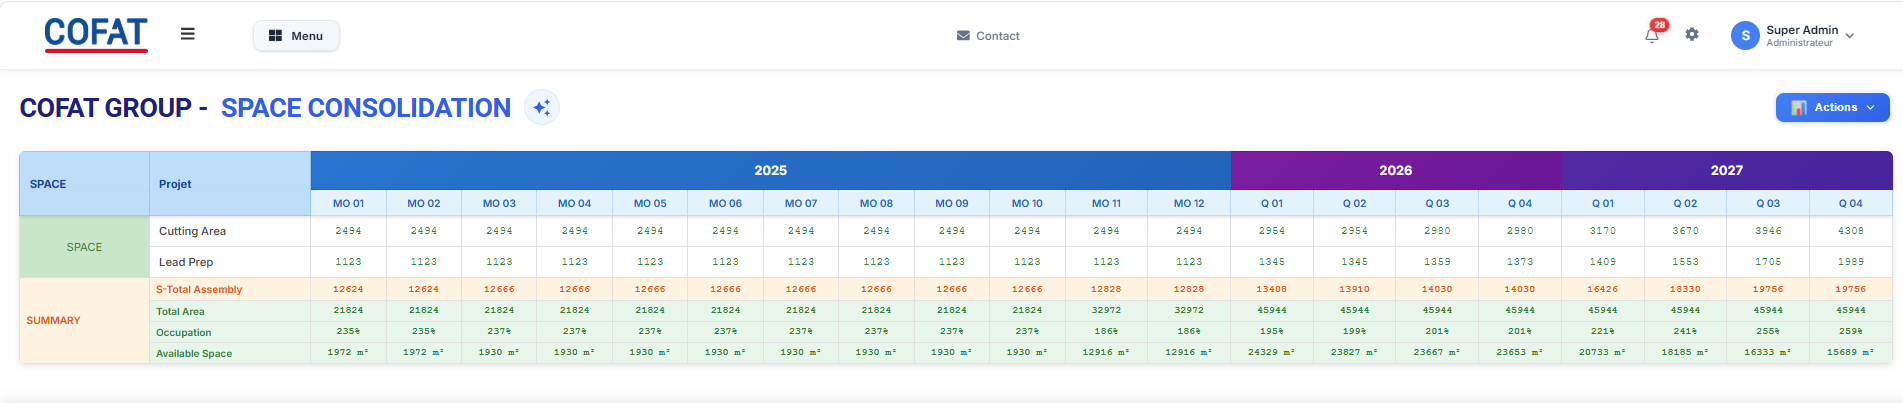
\includegraphics[width=0.9\textwidth]{img/cofat group space consolidation.png}
    \caption{Consolidation mondiale de l'occupation des usines COFAT}
    \label{fig:conso_espaces}
\end{figure}
\vspace{0.5cm}

La Figure \ref{fig:conso_espaces} montre la sommation des surfaces au sol mondiales, par typologie de zone (Coupe, Assemblage). Le graphe consolidé permet à la direction immobilière du groupe de visualiser le taux d'occupation foncier total de COFAT à travers le monde.

\vspace{0.5cm}
\begin{figure}[H]
    \centering
    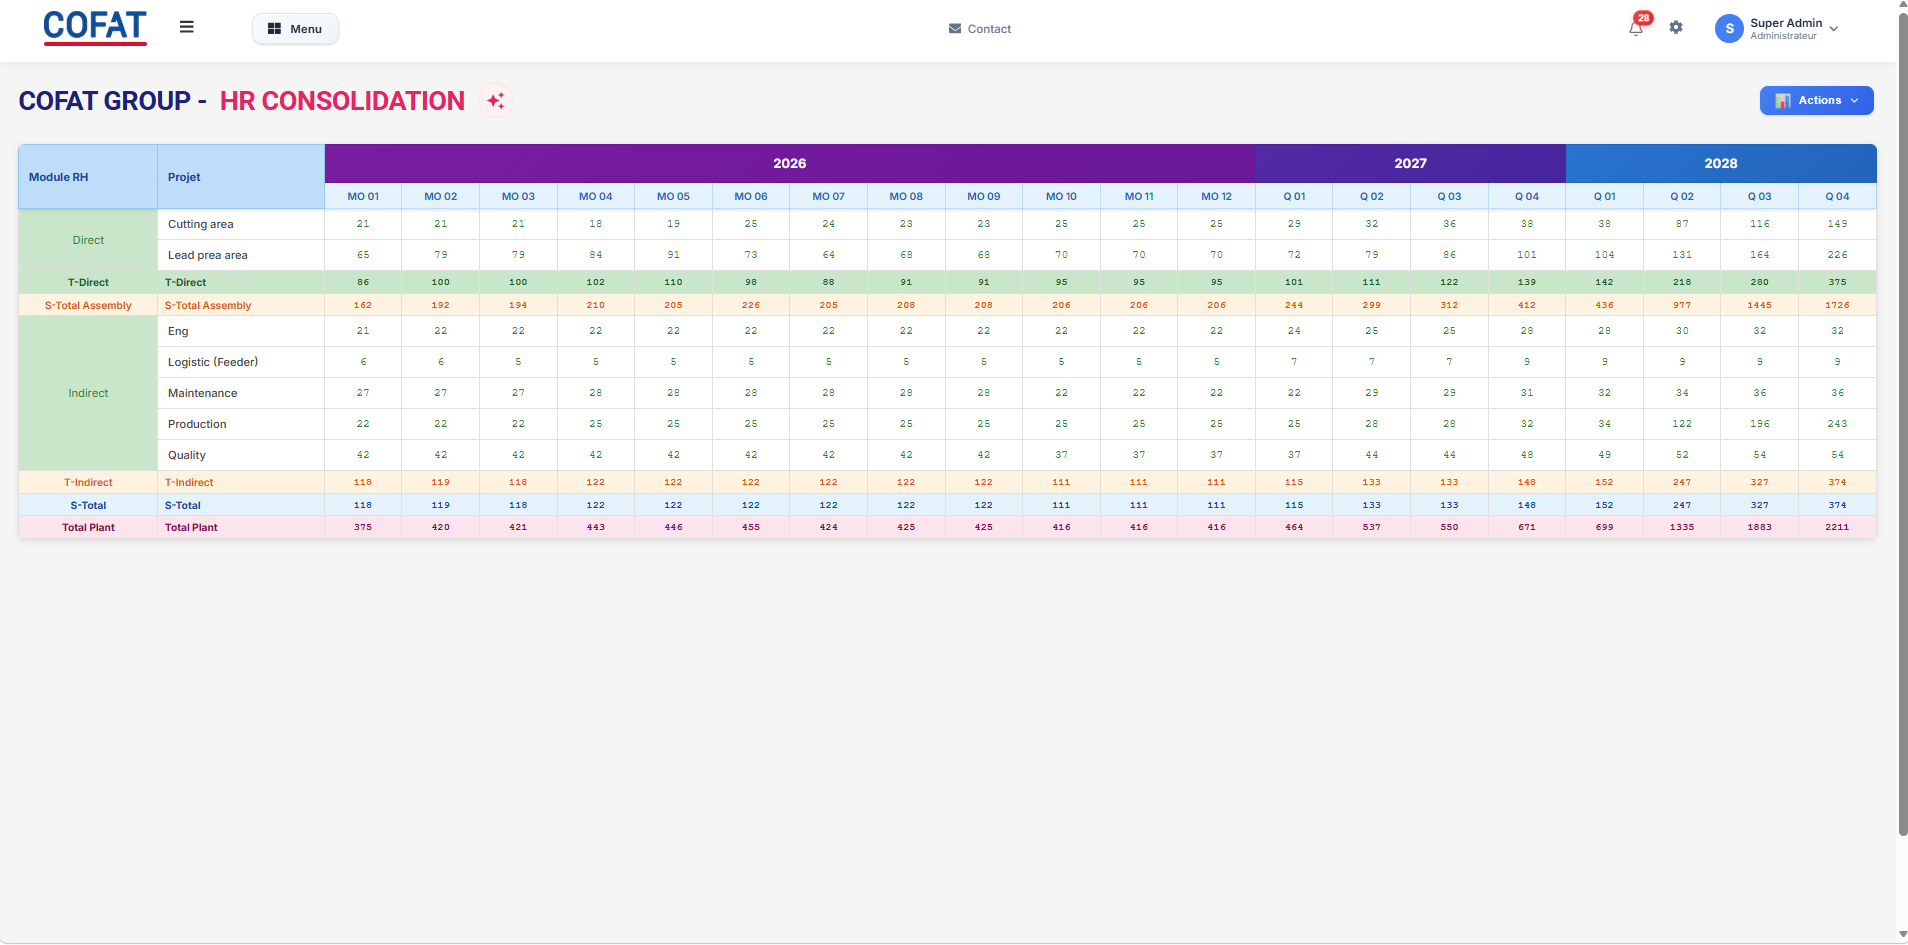
\includegraphics[width=1\textwidth]{img/cofat group HR consolidation.png}
    \caption{Tableau de consolidation RH mondial par projet et catégorie}
    \label{fig:conso_rh_table}
\end{figure}
\vspace{0.5cm}

\vspace{0.5cm}
\begin{figure}[H]
    \centering
    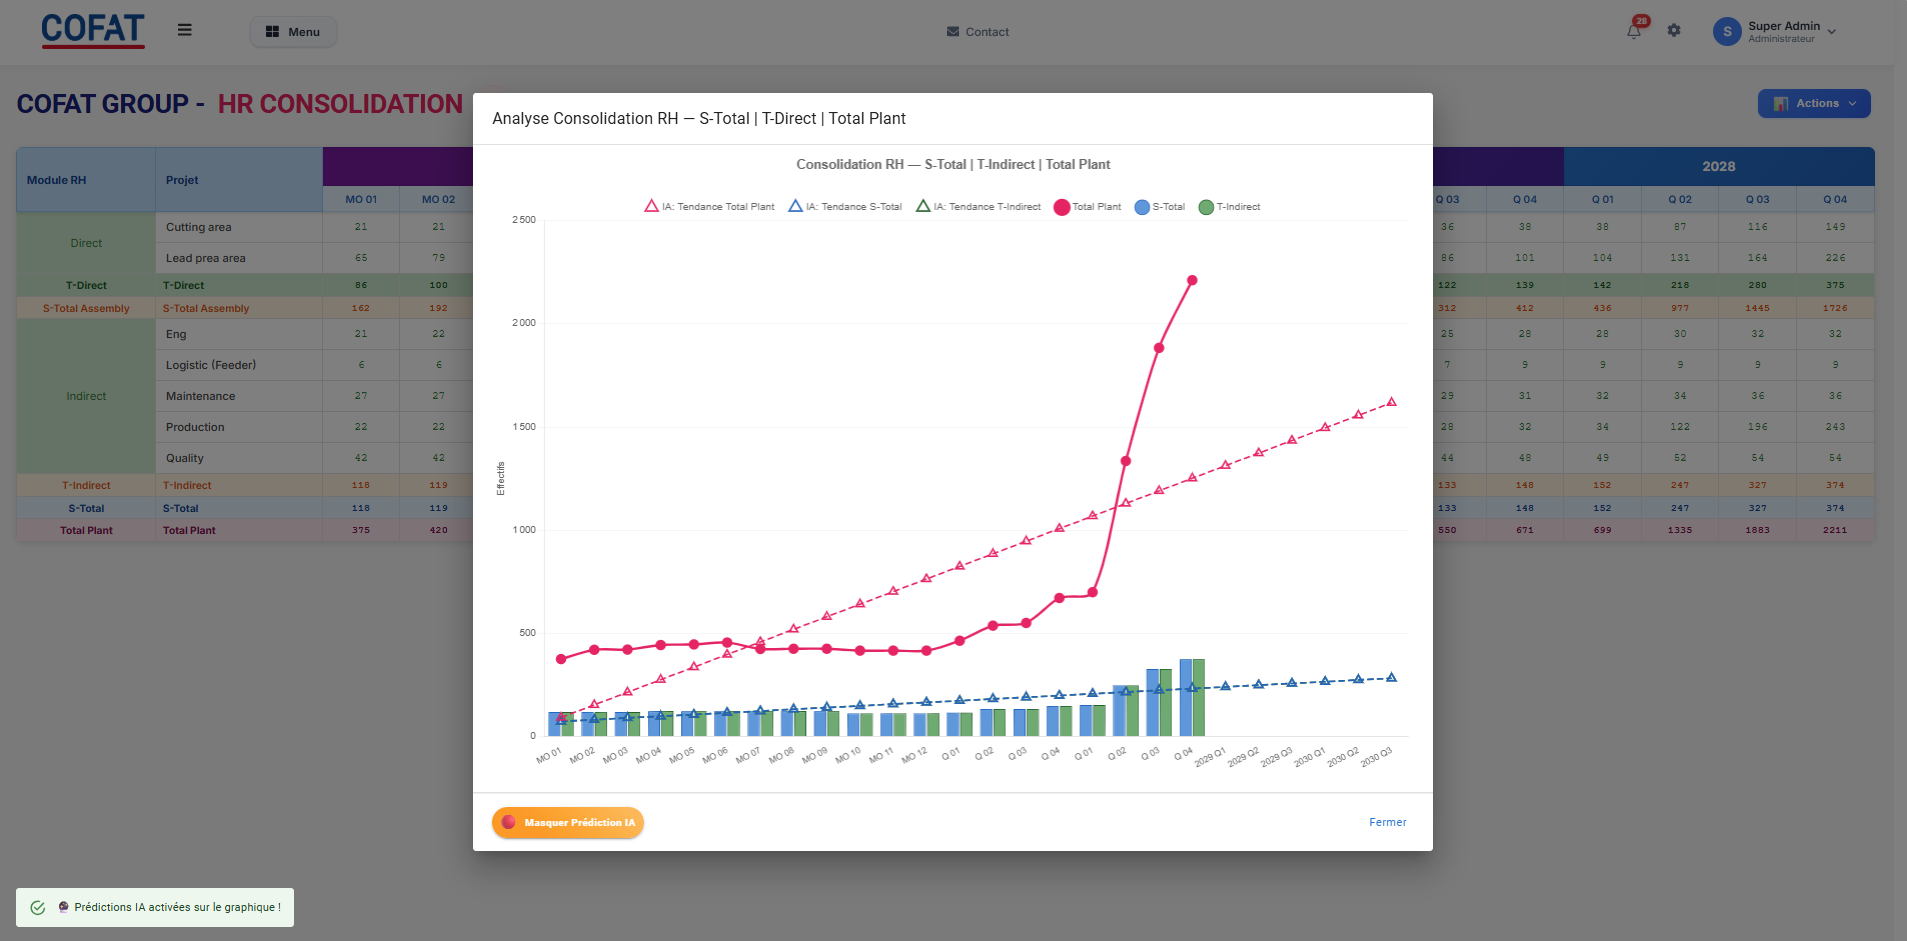
\includegraphics[width=0.9\textwidth]{img/analyse cofat group HR consolidation.png}
    \caption{Dashboard analytique de la montée en charge RH mondiale (Ramp-up)}
    \label{fig:conso_rh_graph}
\end{figure}
\vspace{0.5cm}

\textbf{Analyse de l'agrégation RH (Figures \ref{fig:conso_rh_table} et \ref{fig:conso_rh_graph}) :}
La Figure \ref{fig:conso_rh_table} affiche la somme matricielle des effectifs prévus sur 3 ans (2025-2027) pour les 5 600 employés, fusionnée à partir des 10 sites. 
Pour rendre ce mur de chiffres intelligible, l'application génère automatiquement le Dashboard analytique de la Figure \ref{fig:conso_rh_graph} via \textit{Charts.js}. Ce graphique en barres empilées par période montre l'évolution de la main-d'œuvre nécessaire (par exemple, le pic d'embauche prévu au trimestre Q02 de 2026 pour le démarrage simultané du projet VW Golf 8 en Allemagne et au Mexique). Une courbe de tendance (visible sur la capture d'écran) traverse le graphique, offrant une vision lissée de la trajectoire de recrutement global, facilitant les décisions du DRH du groupe.

Ce module illustre particulièrement bien la valeur ajoutée du passage d'un système décentralisé à une base de données centralisée : la même donnée RH, saisie une seule fois par chaque Site Manager dans son propre périmètre, sert simultanément à trois niveaux de décision différents — le pilotage opérationnel quotidien au niveau du site, la planification des recrutements au niveau du DRH groupe, et la budgétisation prévisionnelle de la masse salariale au niveau de la direction financière — sans qu'aucune ressaisie ni synchronisation manuelle ne soit nécessaire entre ces trois usages.

\textbf{Comparaison avant/après pour la fonction RH Groupe :} avant le déploiement de \textit{Cofat Capacity Study}, le DRH Groupe devait, pour obtenir une vision consolidée des effectifs prévisionnels sur l'ensemble des dix entités, solliciter individuellement chaque responsable RH local, patienter plusieurs jours pour recevoir l'ensemble des retours, puis agréger manuellement des fichiers dont la structure de colonnes différait légèrement d'un site à l'autre en fonction des habitudes locales de chaque responsable RH. Ce délai de plusieurs jours, incompressible dans l'ancien mode de fonctionnement, empêchait de fait toute réactivité face à une variation soudaine de volume de commande nécessitant un ajustement rapide des effectifs sur un ou plusieurs sites. Avec le module de consolidation RH développé lors de ce sprint, cette même vision consolidée mondiale est désormais disponible en quelques secondes, à tout moment, sans aucune sollicitation préalable des équipes locales, celles-ci n'ayant qu'à maintenir leurs propres prévisions à jour au fil de l'eau dans leur module de planification locale.

\subsection{Sécurité et cloisonnement des vues de consolidation}
Un point de vigilance particulier a été apporté à la sécurité de ces vues consolidées, qui exposent par nature une synthèse de données provenant de l'ensemble des dix sites du groupe, y compris des sites concurrents entre eux sur certains segments de marché. Contrairement aux modules de planification locale du Sprint 2, où chaque Site Manager n'accède qu'aux données de son propre site (filtrage systématique par \texttt{siteId} dans chaque requête Sequelize), les routes de consolidation (\texttt{/api/equipment/consolidation}, \texttt{/api/hr/consolidation}, \texttt{/api/spaces/consolidation}) sont exclusivement réservées au rôle Administrateur par le middleware d'autorisation. Un Site Manager authentifié qui tenterait d'appeler directement l'une de ces routes recevrait systématiquement une réponse HTTP 403, quand bien même il connaîtrait techniquement l'URL exacte de l'API. Ce cloisonnement strict garantit qu'aucun responsable d'usine ne puisse consulter, même accidentellement, les niveaux de charge ou les effectifs prévisionnels d'un site concurrent au sein du même groupe.

\section{Le Catalogue : StandardInvestment V2}
Pour calculer les budgets nécessaires aux déficits capacitaires (\textit{toOrder}), il fallait uniformiser les bases de calcul. Si l'usine tunisienne estime une machine de coupe à 150 000 euros via un fournisseur européen, et l'usine brésilienne à 170 000 dollars via un acteur local, la consolidation financière mondiale est biaisée.
Le sprint 3 s'est donc clôturé par la réalisation du module \textit{StandardInvestment V2}, le dictionnaire mondial des prix d'équipements imposé par COFAT.

\textbf{Pourquoi "V2" ?} La dénomination du module fait référence à une nomenclature déjà en usage en interne chez COFAT avant même le lancement de ce projet : une première version du référentiel des équipements standards existait historiquement sous forme de fichier Excel partagé, périodiquement mis à jour par le département Achat central. Le module développé dans le cadre du Sprint 3 en constitue la digitalisation complète, reprenant à l'identique la structure de colonnes déjà connue et validée par les utilisateurs métier, ce qui a permis une adoption immédiate sans phase de formation supplémentaire pour les acheteurs déjà familiers du référentiel V1.

\vspace{0.5cm}
\begin{figure}[H]
    \centering
    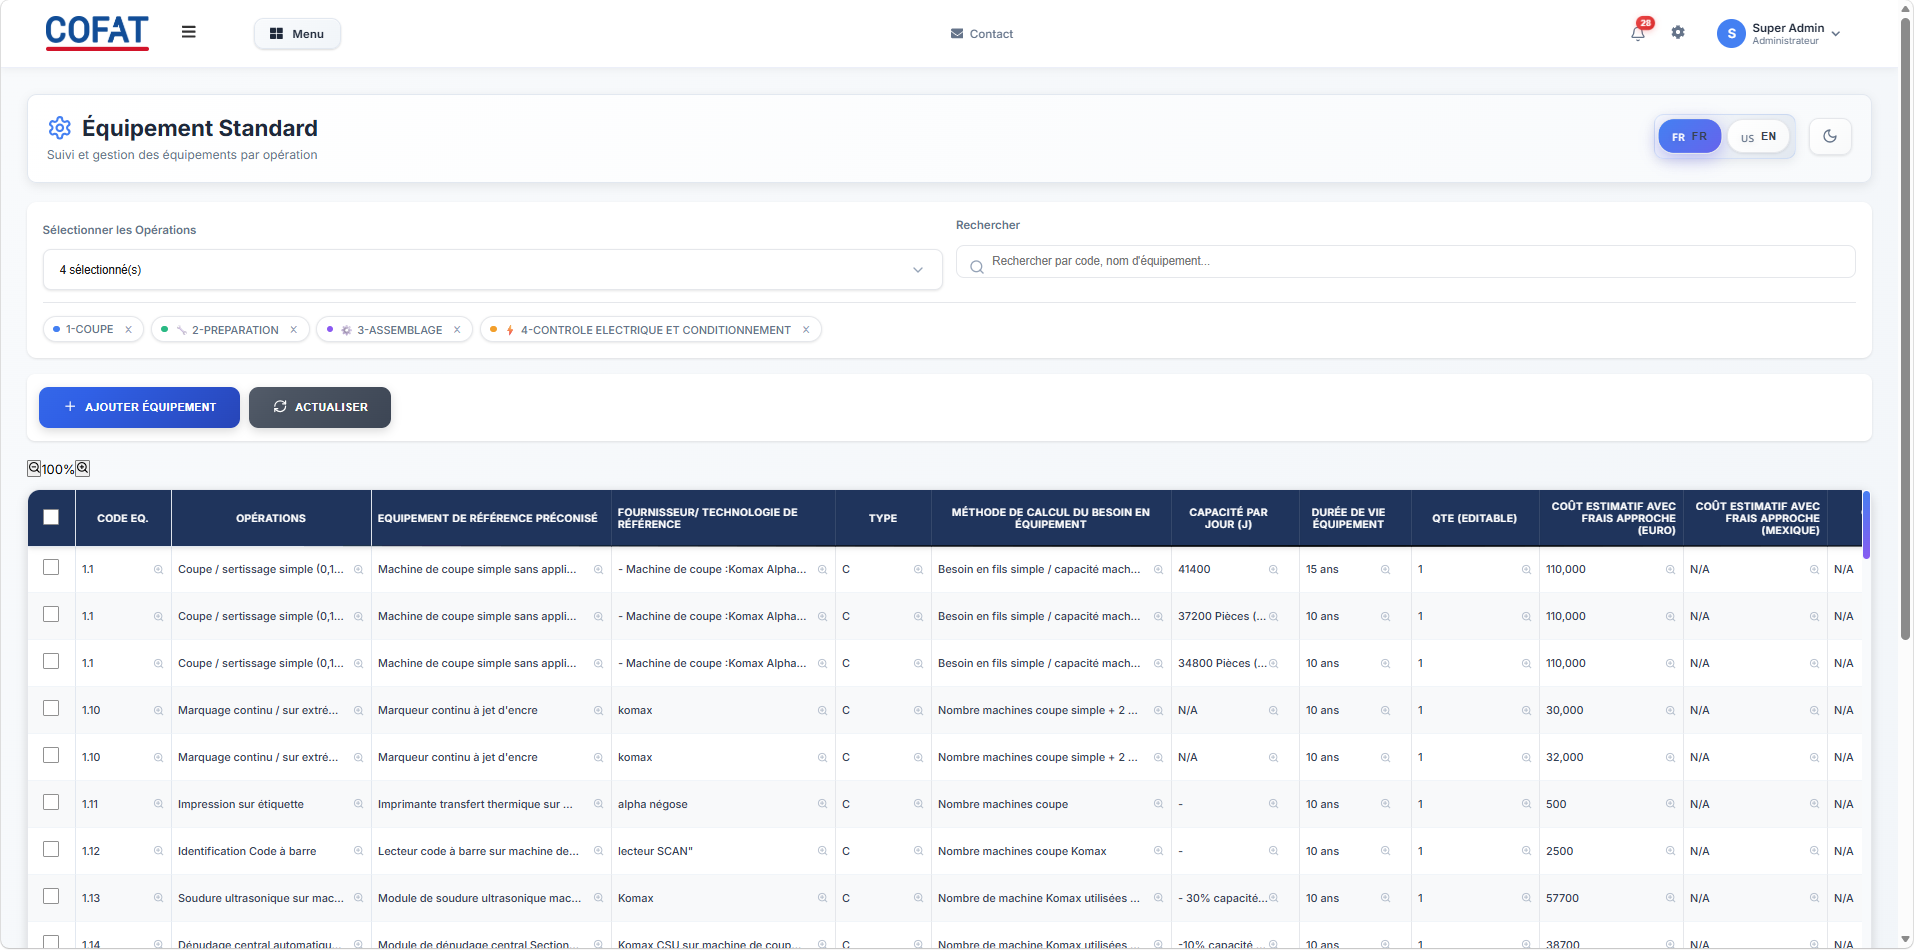
\includegraphics[width=0.9\textwidth]{img/equipement standard.png}
    \caption{Catalogue centralisé StandardInvestment V2}
    \label{fig:standard_equip}
\end{figure}
\vspace{0.5cm}

\textbf{Analyse des champs du modèle de référence (Figure \ref{fig:standard_equip}) :}
L'interface (développée avec la DataGrid de MUI) expose les champs de l'entité SQL \texttt{StandardInvestment}, listant exhaustivement les critères techniques et commerciaux obligatoires d'une machine homologuée :
\begin{itemize}
    \item \textbf{CODE EQ. et TYPE} : Identifiant unique de l'équipement dans l'ERP du groupe.
    \item \textbf{OPERATIONS} : Étape du processus (Coupe, Sertissage).
    \item \textbf{EQUIPEMENT DE REFERENCE PRECONISE} : Modèle exact de la machine (ex: Komax, Schleuniger).
    \item \textbf{FOURNISSEUR/TECHNOLOGIE DE REFERENCE} : Le partenaire industriel homologué.
    \item \textbf{CAPACITE PAR JOUR (J) et DUREE DE VIE} : Paramètres techniques pour calculer l'amortissement.
    \item \textbf{COUT ESTIMATIF AVEC FRAIS APPROCHE (EURO/MEXIQUE/...)} : Les grilles tarifaires par zone géographique.
\end{itemize}

\vspace{0.5cm}
\begin{figure}[H]
    \centering
    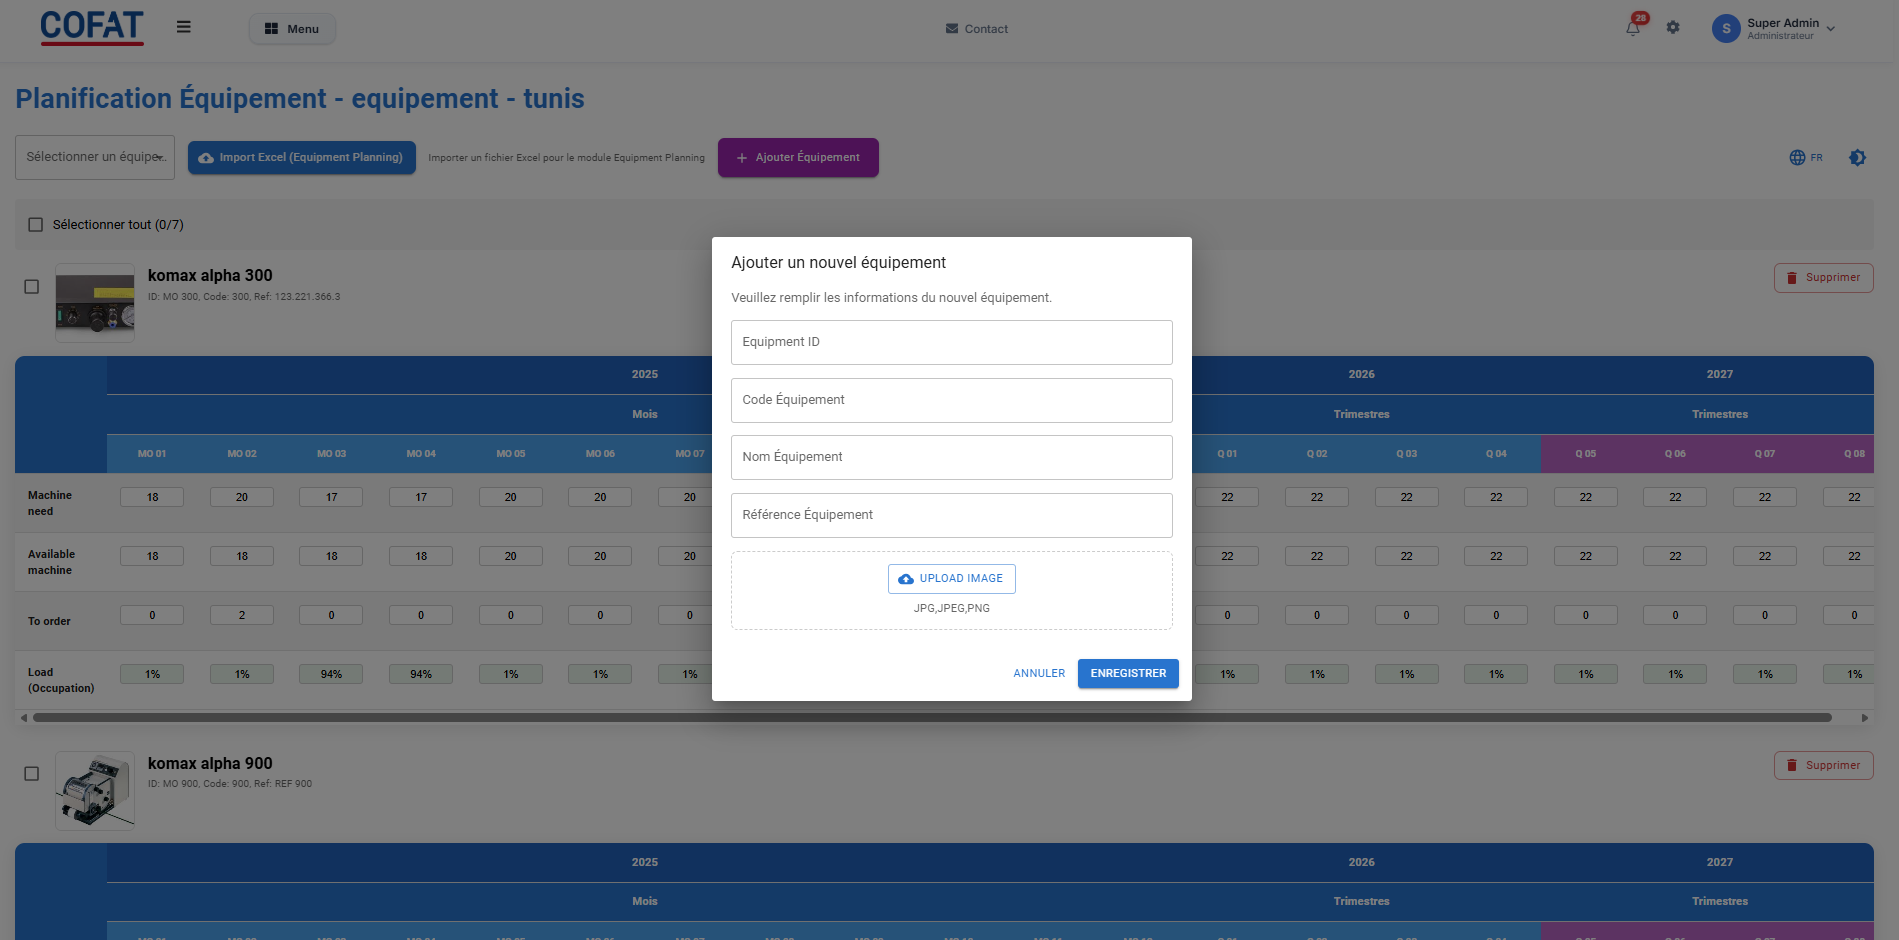
\includegraphics[width=0.8\textwidth]{img/equipement standard ajout 1.png}
    \caption{Formulaire d'ajout d'un équipement standard (Partie 1)}
    \label{fig:add_standard_1}
\end{figure}
\vspace{0.5cm}

\vspace{0.5cm}
\begin{figure}[H]
    \centering
    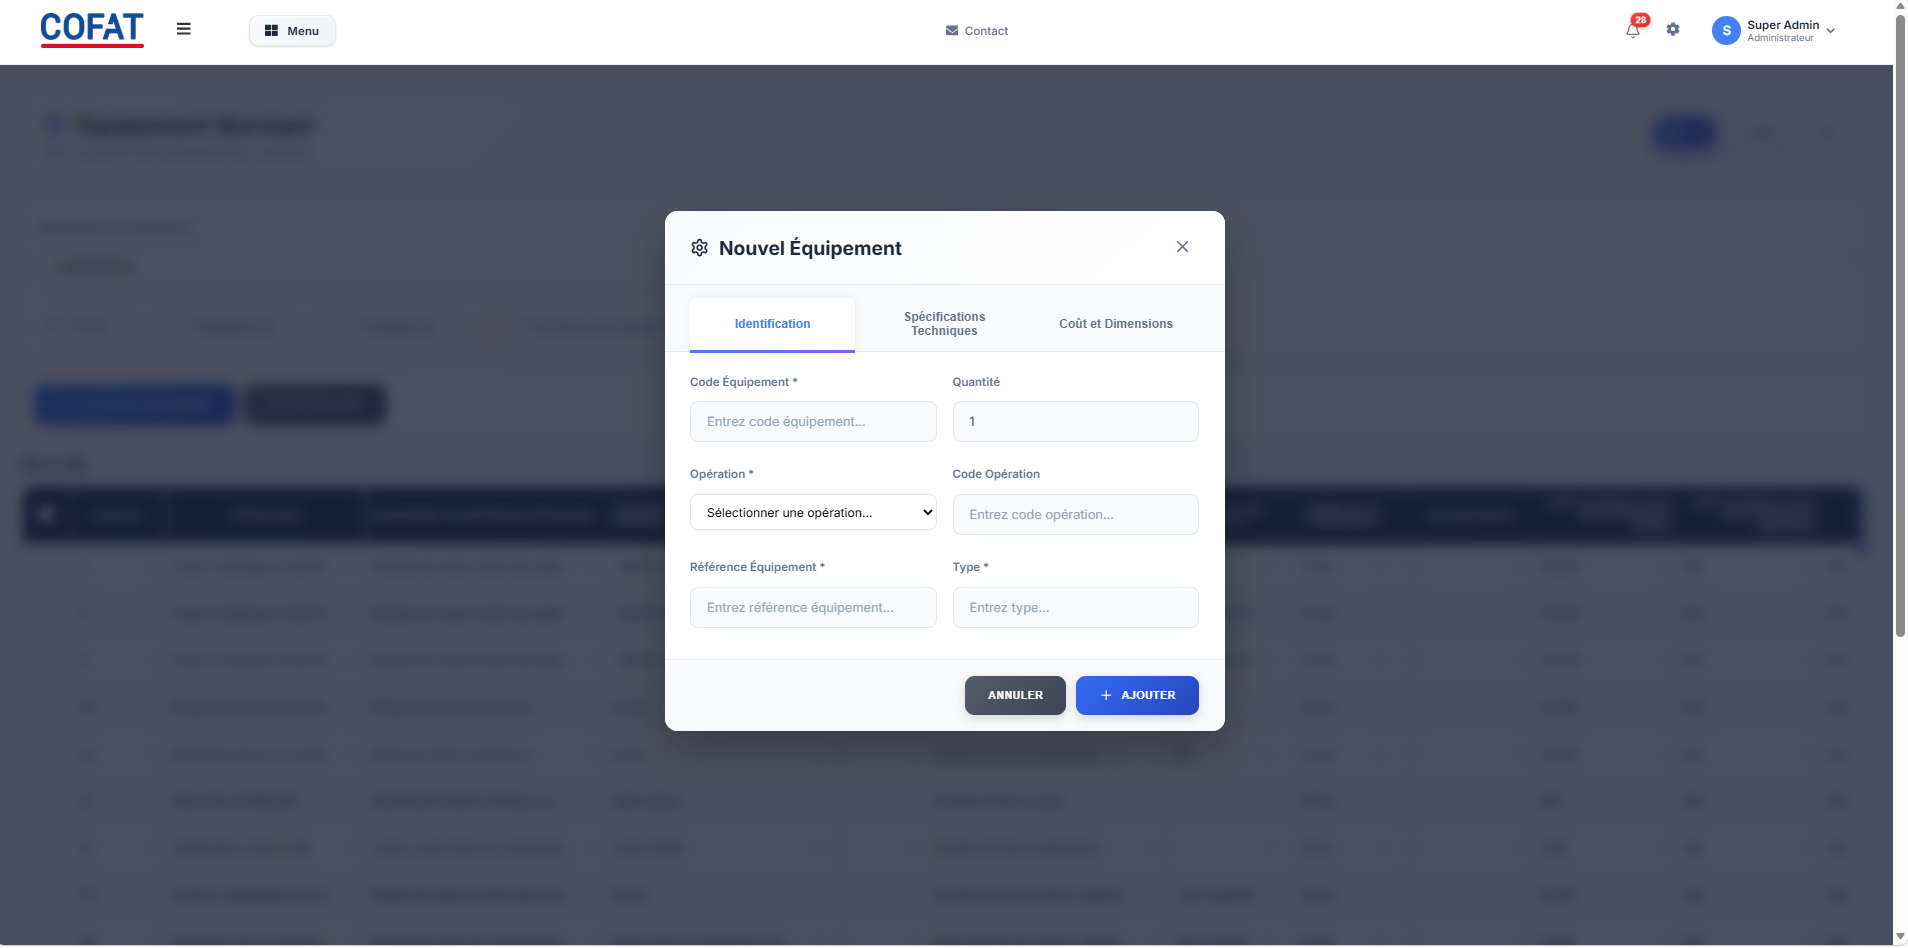
\includegraphics[width=0.8\textwidth]{img/equipement standard ajout 2.png}
    \caption{Formulaire d'ajout d'un équipement standard (Partie 2 : Coûts)}
    \label{fig:add_standard_2}
\end{figure}
\vspace{0.5cm}

\textbf{Gestion des Permissions : L'action de l'Acheteur (Achat) :}
Comme spécifié dans le Chapitre 2, la création (Figures \ref{fig:add_standard_1} et \ref{fig:add_standard_2}) ou la suppression de nouveaux standards est réservée à l'Administrateur central. L'Acheteur (Achat), en tant que négociateur externe, possède des droits précis sur ce catalogue : il est le garant de la justesse des prix affichés. Sa seule action sur ce module est de modifier et mettre à jour les montants dans les colonnes des coûts estimatifs. Ces prix mis à jour sont ensuite utilisés par le système pour monétiser la colonne \textit{toOrder} des planifications locales.

\textbf{Pourquoi plusieurs colonnes de coût par devise plutôt qu'une conversion automatique ?} Le catalogue expose des coûts distincts par zone géographique (EURO pour les fournisseurs européens, coût équivalent pour le Mexique, etc.) plutôt qu'un unique prix de référence converti automatiquement au taux de change du jour. Ce choix reflète une réalité commerciale incontournable : les prix négociés par l'Achat auprès des fournisseurs de machines varient réellement d'une zone à l'autre, en fonction des accords-cadres régionaux, des taxes d'importation locales et des coûts de transport, et ne sont donc pas de simples équivalents monétaires d'un seul et même prix. Stocker un prix unique converti automatiquement aurait masqué ces écarts réels, pourtant essentiels à la bonne prise de décision d'investissement par site.

\vspace{0.5cm}
\begin{figure}[H]
    \centering
    
\includegraphics[width=0.9\textwidth]{img/analyse equipement standard.png}
    \caption{Analyse graphique du catalogue des équipements standards}
    \label{fig:analyse_standard}
\end{figure}
\vspace{0.5cm}

\subsection{Considérations de performance additionnelles}
Au-delà de l'indexation SQL déjà évoquée pour la consolidation des équipements, plusieurs autres leviers de performance ont été mobilisés durant la Release 2 pour garantir une expérience utilisateur fluide malgré le volume croissant de données consolidées.

\textbf{Pagination côté serveur :} les grilles de données Material UI, bien que capables techniquement d'afficher plusieurs milliers de lignes côté client, ont été systématiquement couplées à une pagination gérée côté serveur plutôt que côté navigateur. Concrètement, chaque requête \texttt{GET} vers les routes de planification accepte des paramètres \texttt{page} et \texttt{limit}, et seule la tranche de données demandée est récupérée depuis SQL Server via la clause \texttt{OFFSET/FETCH}, plutôt que de charger l'intégralité de la table en mémoire côté serveur puis de la découper artificiellement. Ce choix, invisible pour l'utilisateur final qui perçoit simplement une navigation fluide entre les pages du tableau, réduit considérablement la charge mémoire du serveur Node.js et le volume de données transitant sur le réseau.

\textbf{Mise en cache légère des référentiels statiques :} certaines données, comme la liste des dix sites du groupe ou le référentiel des types d'équipements, changent très rarement une fois le système en production. Plutôt que d'interroger systématiquement la base de données à chaque affichage d'un menu déroulant utilisant ces référentiels, une mise en cache en mémoire côté serveur (de durée de vie limitée à quelques minutes) a été mise en place pour ces tables spécifiques, réduisant d'autant la pression sur le serveur SQL Server lors des heures de pointe où plusieurs dizaines d'utilisateurs across les dix sites consultent simultanément l'application en début de journée de travail.


La réalisation conjointe des Sprints 2 et 3 a fait émerger plusieurs difficultés d'ingénierie propres à la manipulation de données massives et hétérogènes :

\begin{itemize}
    \item \textbf{Volumétrie des imports Excel.} Certains fichiers RH transmis par les sites de production, notamment ceux couvrant les projets à forte main-d'œuvre comme le VW Tayron, comportaient plusieurs milliers de lignes une fois toutes les catégories et projets combinés. Le traitement synchrone initial de ces fichiers provoquait des temps de réponse HTTP dépassant plusieurs secondes, frisant le \textit{timeout} par défaut du navigateur. La solution a consisté à découper le traitement du fichier en lots (\textit{chunks}) de quelques centaines de lignes, chacun inséré via un appel \texttt{bulkCreate} distinct, réduisant la pression mémoire instantanée côté serveur.
    \item \textbf{Cohérence des unités entre sites.} Lors des premiers tests de consolidation, la nécessité d'une validation stricte du format de saisie des surfaces (en m²) est apparue pour empêcher toute incohérence de fausser silencieusement la consolidation mondiale. Une étape de validation a donc été ajoutée à la logique d'import du module Espaces.
    \item \textbf{Cardinalité des relations dans les agrégations RH.} Le croisement entre catégories de personnel, types de zones et 20 colonnes temporelles (12 mois + 8 trimestres) générait des requêtes de consolidation complexes. Un travail d'optimisation des index composites sur les colonnes \texttt{siteId}, \texttt{type}, \texttt{year} et \texttt{month} de la table \texttt{HR} a été nécessaire pour maintenir des temps de réponse acceptables sur la vue consolidée mondiale.
\end{itemize}

\subsection{Recette fonctionnelle de la Release 2}
Avant la démonstration officielle au Product Owner, une phase de recette interne a été menée sur les trois modules de planification locale et sur les deux modules de consolidation. Cette recette s'est appuyée sur des jeux de données représentatifs importés via la fonctionnalité d'import Excel, afin de confronter l'algorithme à la réalité hétérogène des fichiers de production évoquée précédemment. Chaque module a fait l'objet d'un scénario de test couvrant successivement le cas nominal (fichier bien formé, import réussi), le cas d'erreur partielle (fichier contenant quelques lignes invalides au milieu de lignes valides) et le cas d'erreur totale (fichier au format incorrect, par exemple un fichier \texttt{.csv} renommé en \texttt{.xlsx}). Ces scénarios ont permis de détecter et de corriger, avant la Sprint Review, la plupart des difficultés techniques décrites dans la sous-section précédente. La gestion du code source par branches Git (\textit{feature branches}) a contribué à réduire le risque de régression involontaire d'un module déjà validé lors du développement d'un module suivant.



Le tableau \ref{tab:synthese_release2} récapitule l'état de clôture des User Stories US-04 à US-10, couvrant l'intégralité du périmètre fonctionnel des Sprints 2 et 3.

\begin{table}[h]
\centering
\begin{tabular}{|p{1.6cm}|p{7cm}|p{4.5cm}|p{1.8cm}|}
\hline
\textbf{ID US} & \textbf{Fonctionnalité livrée} & \textbf{Sprint} & \textbf{Statut} \\ \hline
US-04 & Import Excel des équipements locaux & Sprint 2 & Terminée \\ \hline
US-05 & Analyse de charge (Load \%) & Sprint 2 & Terminée \\ \hline
US-06 & Import et analyse RH & Sprint 2 & Terminée \\ \hline
US-07 & Import et gestion des espaces & Sprint 2 & Terminée \\ \hline
US-08 & Dashboard consolidé mondial Équipements & Sprint 3 & Terminée \\ \hline
US-09 & Consolidation Espaces et RH du groupe & Sprint 3 & Terminée \\ \hline
US-10 & Catalogue StandardInvestment V2 & Sprint 3 & Terminée \\ \hline
\end{tabular}
\caption{Synthèse de clôture de la Release 2 (Sprints 2 et 3)}
\label{tab:synthese_release2}
\end{table}

\subsection{Export des vues consolidées}
À l'instar du module de budget non-industriel détaillé au chapitre 5, les trois tableaux de consolidation mondiale (Équipements, Espaces, RH) intègrent chacun une fonctionnalité d'export vers les formats Excel et PDF, réservée au rôle Administrateur. Cette fonctionnalité, bien que techniquement similaire à celle décrite en détail au chapitre suivant (génération côté serveur via la bibliothèque \texttt{xlsx}, transmission sous forme de Blob binaire), présente une particularité propre à la Release 2 : le fichier exporté doit refléter fidèlement la structure matricielle complexe de certains tableaux, notamment la vue RH croisant catégories, projets et vingt colonnes temporelles. La génération du fichier Excel reproduit alors exactement cette structure en figeant les premières colonnes (catégorie, projet) via la fonctionnalité de volets figés d'Excel, afin que la lecture du fichier exporté reste aussi confortable pour un membre du Comité de Direction que la consultation de l'écran correspondant dans l'application.

Cette cohérence entre l'affichage à l'écran et le document exporté, loin d'être un détail cosmétique, a été identifiée comme un critère d'acceptation à part entière lors des ateliers de spécification : les précédents fichiers Excel manuels, bien que sources de nombreux problèmes de fiabilité, avaient au moins l'avantage d'une mise en forme travaillée par leurs auteurs au fil des années. Le nouvel outil ne pouvait se permettre de régresser sur ce point sous peine de rejet par les utilisateurs habitués à des documents visuellement soignés.

\section{Conclusion}
Les Sprints 2 et 3 ont transformé une vision théorique en un outil industriel redoutable.

 Le déploiement des interfaces de planification locale offre enfin aux responsables d'usine l'autonomie et la clarté nécessaires à la gestion de leurs capacités. Le développement minutieux de l'import Excel, traitant validation et injection massive (SQL bulkCreate), garantit une transition numérique sans friction pour les employés habitués aux tableurs.
En capitalisant sur cette base de données fraîchement alimentée, le moteur de consolidation mondiale (Sprint 3) délivre instantanément des tableaux de bord interactifs à la direction. Couplée à la rigueur du catalogue centralisé \textit{StandardInvestment V2}, l'application COFAT Capacity Study permet désormais d'optimiser le parc machine mondial et de prévenir les sous-charges ou surcharges d'usines.
L'étape ultime du projet, couverte par le Sprint 4 (Chapitre 5), consistera à numériser le circuit d'approbation financière à travers un workflow dynamique dédié aux budgets non-industriels.